\documentclass[12pt,a4paper]{article}
\usepackage[warn]{mathtext}
\usepackage[utf8]{inputenc}
\usepackage[T2A]{fontenc}
\usepackage[english,russian]{babel}
\usepackage{indentfirst}
\usepackage{misccorr}
\usepackage{subcaption}
\captionsetup{compatibility=false}
\usepackage{geometry}
\geometry{verbose,a4paper,tmargin=2cm,bmargin=2cm,lmargin=1.5cm,rmargin=1.5cm}
\usepackage{graphicx}
\usepackage{wrapfig}
\usepackage{amsmath}
\usepackage{fancyhdr}
\usepackage{floatflt}
\usepackage{float}
\usepackage{amssymb}
\usepackage{color}
\usepackage{lscape}
\usepackage{hvfloat}
\usepackage{amsfonts}
\usepackage{euscript}

\begin{document}

\begin{titlepage}
	\centering
	\vspace{5cm}
	{\scshape\LARGE Московский физико-технический институт \par}

	\vspace{3cm}
	{\scshape\Large Лабораторная работа № 4.7.3 \par}
	\vspace{1cm}
	{\huge\bfseries  Изучение поляризованного света\par}
	\vspace{1cm}
	\vfill
\begin{flushright}
	{\large Выполнила студентка группы Б01-903}\par
	\vspace{0.3cm}
	{\LARGE Прохорова Юлия}
\end{flushright}
	
	\vfill

% Bottom of the page
	Долгопрудный, 2020 г.
\end{titlepage}



\newpage

\tableofcontents

\newpage

\newcommand{\RNumb}[1]{\uppercase\expandafter{\romannumeral #1\relax}}

\pagestyle{fancy} 
\fancyhead{} 
\fancyhead[RE,RO]{\thepage} 

\fancyhead[LO,LE]{Юлия Прохорова}

\fancyfoot{}

\section{Цель работы} 

Ознакомление с методами получения и анализа поляризованного света. 
 
 
\section{Оборудование}
Оптическая скамья с осветителем, зеленый светофильтр, два поляроида, черное зеркало, полированная эбонитовая пластинка,
 стопа стеклянных пластинок, слюдяные пластинки разной толщины, пластинки толщиной $\lambda/4$ и $\lambda/2$, пластинка
  в одну длину волны для зеленого света (пластинка чувствительного оттенка).

\section{Теоретическая часть}

\subsection{Определение направления разрешенной плоскостиколебаний поляроида.}

	\

	Определить направление разрешенных колебаний поляроида проще всего с помощью черного зеркала.
	При падении света на отражающую поверхность под углом Брюстера, свет в отраженном луче почти полностью поляризован, а вектор $ \vec{E}$ параллелен отражающей поверхности. Луч свеа, прошедший поляроид и отразившийся от черного зеркала,
	имеет минимальную интенсивность при выполнении двух условий: во-первых, свет падает на отражающую поверхность под углом Брюстера и, во-вторых, в падающем пучке вектора $\vec{E}$ лежит в плоскости падения.

	\

	Вращая поляроид вокруг направления луча и черное зеркало вокруг оси, перпендикулярной лучу, методом последовательных приближений можно добиться минимальной яркости луча, отраженного от зеркала,
	и таким образом определить разрешенное направление поляроида.

	\

	Измеряя угол поворота (угол Брюстера), нетрудно определить коэффициент преломления материала, из которого изготовлено зеркало. Описанный метод часто используется для измерения коэффициента преломления прозрачных диэлектриков.

\subsection{Получение эллиптически поляризованного света.}

\begin{wrapfigure}[]{r}{130pt}
	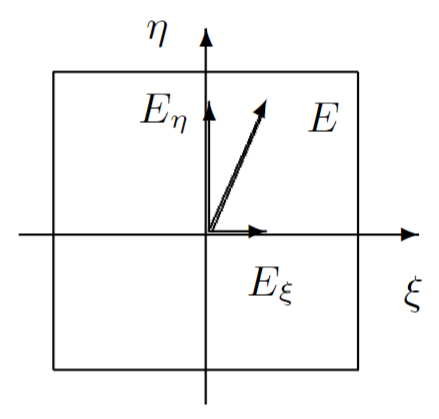
\includegraphics[scale = 0.3]{razl.png}
	\caption{Разложение линейно поляризованного света по главным направлениям двоякопреломляющей пластинки}
	\label{p10}
	\end{wrapfigure}

	Эллиптически поляризованный свет можно получить из линейно поляризованного с помощью двоякопреломляющих кристалличесих пластинок.

	\

	Двоякопреломляющая пластинка имеет два взаимно перпендикулярных главных направления, совпадающих с осями эллипсоида диэлектрической проницаемости. Волны, поляризованные вдоль главных направлений, распространяются в пластинке с разными скоростями, не изменяя характера своей
 поляризации. Эти волны называют главными. Пусть x, y - главные направления кристаллической пластинки, тогда $n_x  и n_y$ - показатели преломления для главных волн.

 \

 Пусть на пластинку падает линейно поляризованная волна, электричекий вектор которой ориетнирован под некоторым углом $\alpha$ к оси х.
 Разложим вектор $\vec{E}$  на $\vec{E_x} и \vec{E_y}$ находятся в фазе. На выходе из-за разности скоростей между ними появляется разность хода $d(n_x - n_y)$, при этом сдвиг фаз определяется соотношением 

 \begin{equation}
	 \varDelta\varphi = \frac{2\pi}{m} = kd(n_x - n_y) 
 \end{equation}

 Как уже отмечалось, при сложении двух взаимно перпендикулярных колебаний, обладающих некоторым сдвигом фаз, образуется колебание, поляризованное по эллипсу.

 

 Рассмотрим практически важные частные случаи.
 \begin{itemize}
	 \item Пластинка (в длину волны $\lambda$) дает сдвиг фаз $2\pi$. В результате сложения волн на выходе пласинки образуется линейно поляризованная волна с тем же направлением колебаний, что в падающей волне.
	 \item Пластинка дает сдвиг фаз $\pi$ (полдлины волны $\lambda/2$). Н выходе пластинки снова образуется линейно поляризованная волна. Направление $bb'$ колебаний этой волны повернуто относительно направления $aa'$ колебаний падающей волны. Как нетрудно сообразить, направление $bb'$ является зеркальным отображением направления $aa'$ относительно одного из главных направлений пластинки. Такую пластинку изпользуют для поворота направления колебаний линейно поляризованного света.
	 \item Пластинка создает между колебаниями фаз $\pi/2$ (пластинка в четверть длины волны). При сложении двух взаимно перпендикулярных колебаний, имеющих разность фаз $\pi/2$, образуется эллипс, главные оси которого совпадают с координатными осями x и y. При равенстве амплитуд возникает круговая поляризация.
 \end{itemize} 

 \begin{wrapfigure}[13]{r}{130pt}
	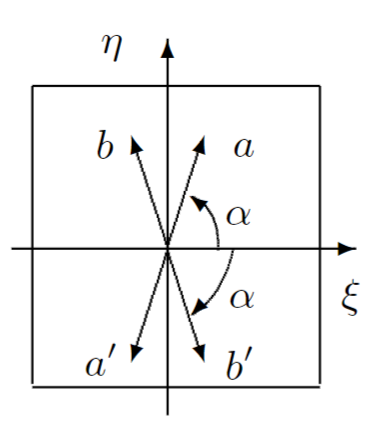
\includegraphics[scale = 0.3]{turn.png}
	\caption{Поворот направления колебаний с помощью пластинки в $\lambda/2$}
	\label{p10}
	\end{wrapfigure}

 Следует отметить, что, говоря о прастинках $\lambda, \lambda/2, \lambda/4$ и тд, взегда подразумевают какую-либо монохроматическую компоненту (например, $\lambda/2$ для зеленого света). Если на двояко преломляющую пластинку падает не хроматический свет, то на выходе из нее для разных спектральных компонент эллипсы поляризации будут различны.
 

 \subsection{Анализ эллиптически поляризованного света}
 Анализ эллиптически поляризованного света сводится к нахождению главных осей эллипса поляризациии к определнию направления вращения электрического вектора.
 
 \

 Главные оси эллипса поляризации определяются с помощью анализатора по максимуму и минимуму интенсивности проходящего света. Направление вращения электрического вектора может быть найдено с помощью пластинки в четверть длины волны, для которойизвестно, какая из главных волн, $E_x$ и $E_y$, имеет большую скорость распространения (соответственно меньшее значение показателя преломления).

\

Выберем для определенности координаты оси x и  y на пластинке так, чтобы $n_x < n_y$. В этом случае главная волна $E_x$ имеет большую скорость распространения. Поместим такую пластинку на пути эллиптически поляризованного света и совместим главные направления пластинки $\lambda/4$ с главными осями эллипса поляризации. На выходе из этой пластинки сдвиг фаз между $E_x$  и $E_y$ вместо $\pi/2$ станет равным нулю или $\pi$. Свет окажется линейно поляризованным. Из двух возможных значений сдвига фах (0 и $\pi$) реализуется одно: то, которе соответствует имеющемуся в волне направлению вращения электрического вектора.

\  

Рассмотрим, например, случай, когда электрический вектор в эллиптически поляризованной волне вращается против часовой стрелки, если смотреть навстречу лучу. В этом случае в волне, падающей на плстинку в $\lambda/4$, колебание $E_y$ отстает по фазе на $\pi/2$ от колеабния $E_x$. При прохождении через
 пластинку разность фаз увеличивается до $\pi$. Таким образом, на выходе из пластинки возникают линейно поляризованные волны со сдвигом фаз $\pi$. Сложение этих волн дает плоскополяризованную волну, электрический вектор которой располагается во втором и четвертом квадратнах координатной плоскости.

 \

Рассуждая аналогичным образом, найдем, что при вращении электрического вектора по часовой стрелке направление колебани в линейно поляризованной волне, выходящей из пластинки,
располагается в первом и третьем квадратнах. Определяя направление колебаний на выходе из плсатинки с помощью поляроида, можно, таким образом, определить характер эллиптической поляризации (вращение против или по часовой стрелке). 

\subsection{Пластинка чувствительного оттенка}


\begin{wrapfigure}[13]{r}{130pt}
	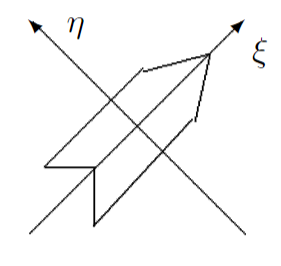
\includegraphics[scale = 0.3]{пластинка_чувствительная.png}
	\caption{Пластинка чувствительного оттенка}
	\label{p10}
	\end{wrapfigure}

Выше предполагалость известным, какому из двух главных направлений пластинки в четверть длины соответствует большая скорость распространения света. Установить  это можно различными способами, например, с помощью пластинки чувствительного оттенка (пластинку в $\lambda$ для зеленой спектральной компоненты, $\lambda = 560 нм$).

\

Пластинка имеет форму стрелы, вдоль оси которой расположено главное направление, соответствующее большей скорости распространения. 

\

Если пластинка чувствителного оттенка помещена между скрещивающими поляроидами, и главные направления пластинки не параллельны направлениям разрешенных колебаний поляроидов, то при освещении белым светом пластинка кажется окрашенной в лиловый цвет. Это объясняется тем, что что зеленая компонента линейно поляризованного света при прохождении пластинки не меняет поляризации и задерживается вторым поляроидом. Для красной и фиолетовой компонент пластинка создает сдвиг фаз, несколько отличный от $2\pi$. На выходе из пластинки  красная и фиолетованя компоненты оказываются поэтому эллиптически поляризованными и частично проходят через второй поляроид. Таким образом, в известном смысле наблюдаемый в указанном опыте цвет пластинки дополнителен к зеленому.

\


Если у пластинки чувствительного оттенка и пластинки $\lambda/4$ \textbf{совпадут главные направления}, соответствующие \textbf{большей скорости распространения}, то разность хода между $E_x$ и $E_y$ для зеленого света составит уже $5\lambda/4$. Это соответсвует разности хода в $\lambda$ для света с большей длиной волны (для более красного). При освещении пластинок белым светом теперь погасится не зеленая, а красная часть спектра, проходящий свет будет казаться зеленовато-голубым.

\

Если же главные направления, соответсвующие большей скорости \textbf{окажутся перпендикулярными}, то проходящий свет приобретет оранжево-желтую окраску (погасится фиолетово-голубая часть спектра). 

Получим: $\lambda - \lambda/4 = 3\lambda/4 = \lambda' < \lambda $ следует, что $P_2$ не пропускает голубой свет. 

Показатель преломления для обыкновенной волны, которая распространяется вдоль оптической оси $x$, будет меньше, чем для необыкновенной ($n_o < n_e$) следовательно скорость будет больше.

\subsection{Интерференция поляризованных лучей}

\begin{wrapfigure}[13]{r}{130pt}
	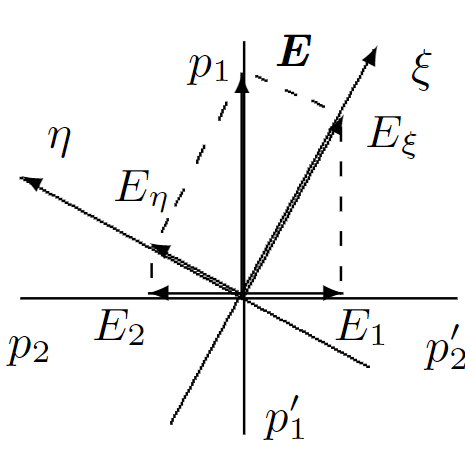
\includegraphics[scale = 0.3]{интерференция.png}
	\caption{К объяснению интерференции поляризованных лучей}
	\label{p10}
	\end{wrapfigure}


Тонкие двоякопреломляющие пластинки, помещенные между поляроидами, кажутся окрашенными. Эта окраска может быть истолкована как результат интерференции поляризованных лучей.

\

Здесь $p_1p'$ - разрешенное направление колебаний поляризатора (первого поляроида); x, y - координатная система, связанная с главными направлениями двоякопреломляющей пластинки; $p_2p'$ - разрешенное направление колебаний анализатора (второго поляроида). Волна $E_x$ и $E_y$ на выходе из пластинки когерентны, но не могут интерферировать, так как $E_x \perp E_y$. Волны $E_1$ и $E_2$ на выходе второго поляроида также - когеренты и поляризованы в одной плоскости в добавок. Эти волны интерферируют между собой. Результат интерференции зависящим от длины волны сдвигом фаз между $E_1$  и $E_2$. В результате интерференции поляризованных лучей пластинка, освещенная белым светом, кажется окрашенной.

Если поворачивать двояко преломляющую пластинку, расположенную между скрещенными поляроидами, то соотношение амплитуд волн $E_1$ и $E_2$ и разность фаз между ними не изменяются. Это означает, что цвет пластинки при ее поворотах не меняется, а меняется только интенсивность света. За один оборот пластинки интенсивноть4 раза обращается в нкль. Это происходт при совмещении главных направлений с разрешенными направлениями колебаний поляроидов.

\

Если же двоякопреломляющую пластинку оставить неподвижной, а второй поляроид повернуть, так, чтобы разрешенные направления $p_1p'$ и $p_2p'$ совпали, то волны $E_1$ и $E_2$ приобретаютдополнительный фазовый сдвиг на $\pi$ для всех спектральных компонент; при этом их амплитуды изменяются так, что цвет пластинки изменится на дополнительный.
\section{Ход работы}

\subsection{Определение разрешенных направлений поляроидов}


\begin{enumerate}
\item
Разместим на оптической скамье осветитель $S$, поляроид $P_1$ и черное зеркало как на рис. \ref{p1}
\item

Поворачивая поляроид добьемся наименьшей яркости отраженного пятна и определим разрешенное направление. $\varphi_1\approx 127^\circ$

\begin{figure}[H]
\begin{center}
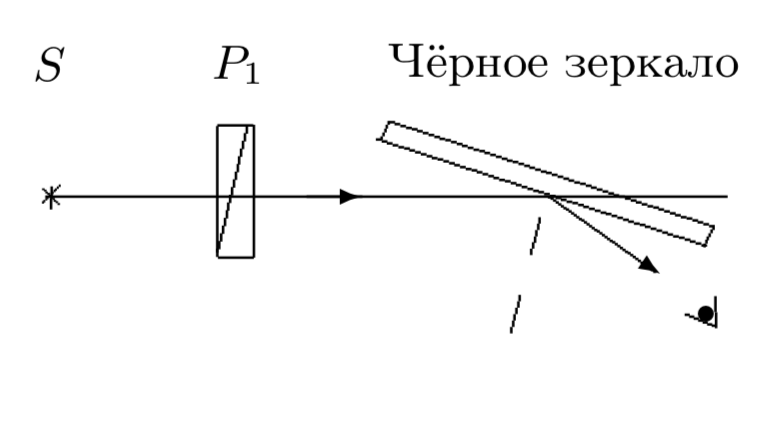
\includegraphics[scale = 0.4]{p1.png}
\caption{Определение разрешенного направления поляроида}
\label{p1}
\end{center}
\end{figure}

\item
Поставим вместо черного зеркала - второй поляроид. Скрестив поляроиды, определим разрешенное направление второго. $\varphi_2 \approx 50^\circ$
\end{enumerate}

\subsection{Оценим угол Брюстера и коэффициент преломления для эбонита}

\begin{enumerate}
\item
Поставим на скамью эбонитовую пластинку и определим по лимбу угол Брюстера для эбонита.  $\varphi_{\text{Б}} \approx 123^\circ$

\item
Добавим светофильтр Ф. $\varphi_{\text{Б}} \approx 125^\circ$
\item
Расчитаем показатель преломления по формуле $\tg{(\varphi_{\text{Б}})} = n$, получим: $n \approx 1.54 $ $n_{\text{фильтр}} \approx 1.43$

\end{enumerate}

\subsection{Исследуем характер поляризации света в преломленном и отраженном от стопы лучах}

Для этого поставим вместо эбонитового зеркала (рис. \ref{p1}) стопу стеклянных пластинок под углом Брюстера. 

\begin{wrapfigure}[10]{l}{130pt}
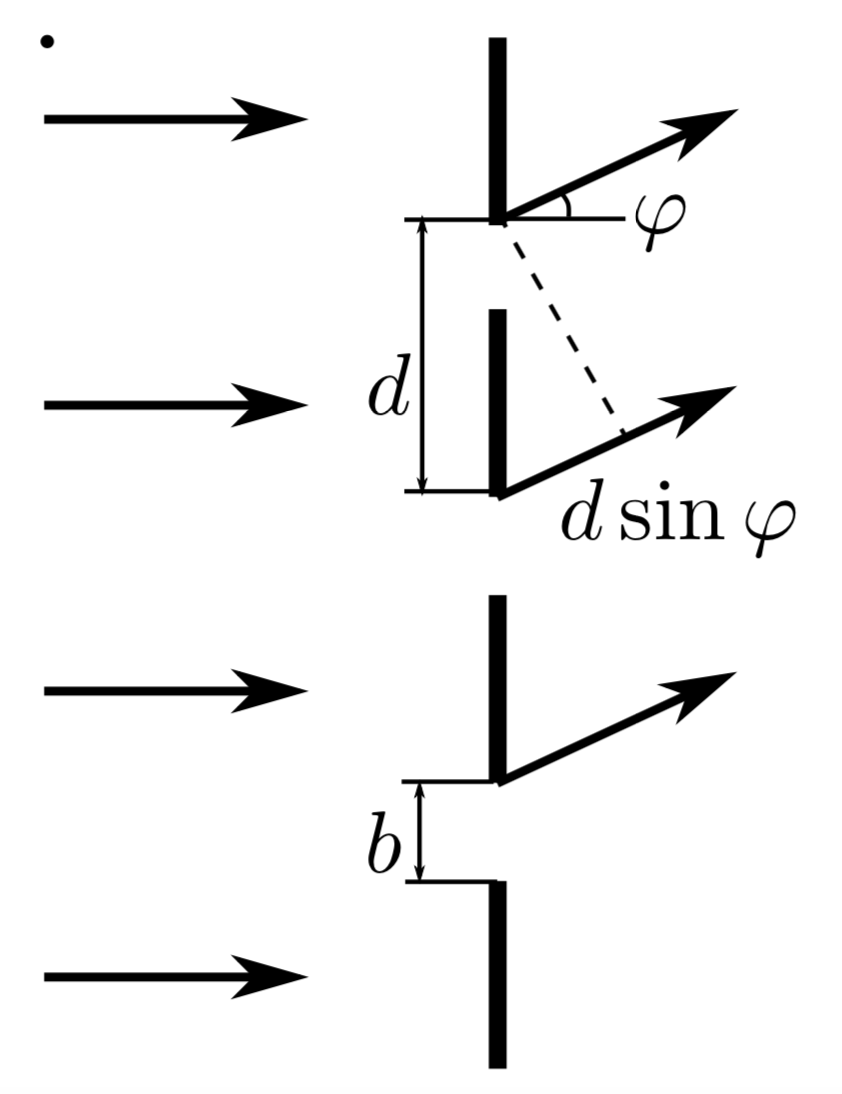
\includegraphics[scale = 0.3]{p2.png}
\caption{Исследование стопы}
\label{p2}
\end{wrapfigure}

Освятим стопу неполяризованным светом и, рассматривая через поляроиды (рис. \ref{p2}) отраженный и преломленный лучи, определим в них орейнтации вектора $\vec{E}$. 

Видим, что плоскости поляризации для отраженного и преломленного лучей взаимно перпендикулярны. Преломленные лучи горизонтальные, отраженные - вертикальные. Лучи имеют правый вид поляризации. ($\vec{E}$ вращается по часовой стрелке - значит правая)
(В отраженном луче преобладают колебания, перпендикулярные плоскости падения; в преломленном луче преобладают колебания, параллельные плоскости падения)

\subsection{Определим главные направления двояко преломляющих пластин}

Поставим кристаллическую пластинку между скрещенными поляроидами (рис. \ref{p3})

\begin{wrapfigure}[9]{r}{130pt}
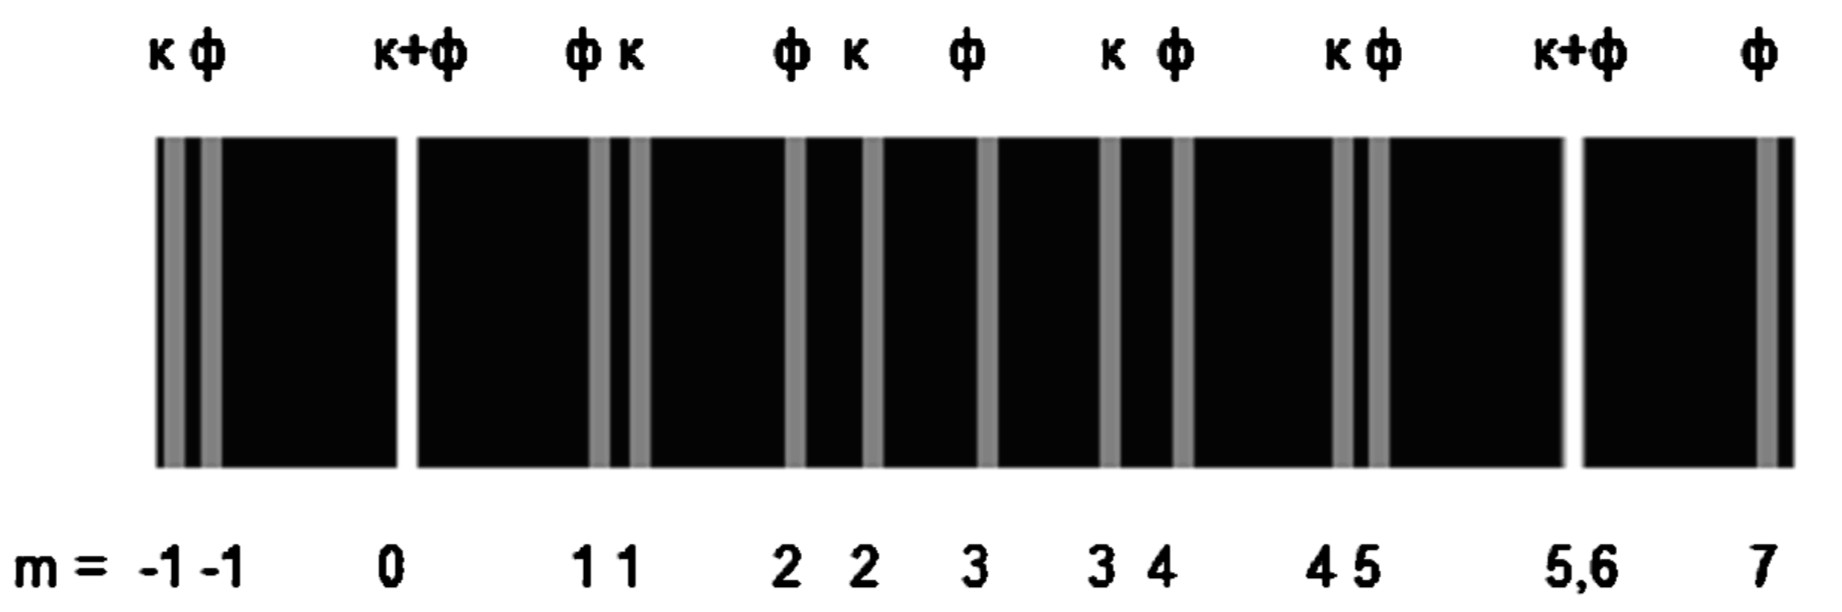
\includegraphics[scale = 0.3]{p3.png}
\caption{Определение главных направлений в пластинках}
\label{p3}
\end{wrapfigure}

Вращая пластинку вокруг направления луча и наблюдая за интенсивностью света, проходящего сквозь второй поляроид, определим  при каком условии главные направления пластинки совпадают с разрешенными направлениями поляроидов. 

При максимальной интенсивности разрешенные направления поляроидов совпадают с главными осями пластинки. 
\par
Для 1-ой поастинки углы : $60^\circ , 148^\circ, 236^\circ, 325^\circ$.
\par
Для 2-ой поастинки углы : $64^\circ , 152^\circ, 240^\circ, 332^\circ$.

\subsection{Выделение пластинок $\lambda/4 $ и $\lambda/2$}

Добавим к схеме (рис. \ref{p3}) зеленый фильтр. Установим разрешенное направление первого поляроида горизонтально, а главные направления исследуемой пластинки - под углом $45^\circ$ к горизонтали. С помощью второго поляроида установим, какую поляризацию имеет свет, прошедший пластинку. 

\begin{itemize}
\item
$\lambda/4$ создает сдвиг фаз между колебаниями - эллиптическая поляризация. Она не меняет интенсивность при повороте.

\item
$\lambda/2$ не меняет характер поляризации, при ее повороте меняется интенсивность. 
\end{itemize}

\subsection{Определить быструю  медленную оси в пластинке $\lambda/4$}

Поставим между скрещенными поляроидами пластинку чувствительного оттенка, имеющую вид стрелки (она не меняет поляризацию зеленого света)

\begin{wrapfigure}[11]{l}{130pt}
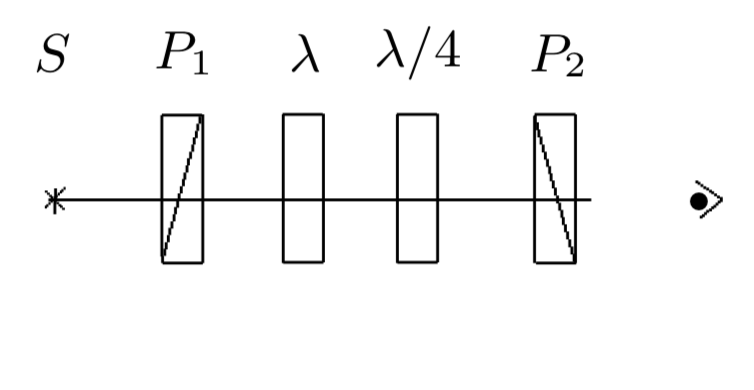
\includegraphics[scale = 0.3]{p4.png}
\caption{Определение направлений большей и меньшей скорости}
\label{p4}
\end{wrapfigure}

Если мы уберем зеленый фильтр, то стрелка окрасится в пурпурный цвет. Зеленый свет задерживается вторым поляроидом, а красная и синяя компоненты проходят. 

При повороте рейтера со стрелкой на $180^\circ$ вокруг вертикальной оси цвет стрелки меняется от зелено-голубого до оранжево-желтого. 

Добавим в схему пластинку  $\lambda/4$ (рис. \ref{p4}), главные направления которой совпадают с главными направлениями пластины $\lambda$ и ориентированы под углом $45^\circ$ к разрешенным направлениям скрещенных поляроидов. 


Если же главные направления пластинки $\lambda$ не параллельны направлениям разрешенных колебаний скрещенных поляроидов, то пластинка окрасится в лилово-красный цвет, потому что зеленая компонента линейно поляризованного света при прохождении пластинки не меняет поляризации и задерживается вторым поляроидом. 

Уберем пластинку чувствительного оттенка. Быстрая ось получилась на $148^\circ$.


\subsection{Интерференция поляризованных лучей} 

Разместим между скрещенными поляроидами мозаичную слюдяную пластинку. Она собрана из 4х полосок слюды (две по $\lambda/4 $ и по одной - $\lambda/2$ и $3\lambda/4$). В центральном квадратике нет слюды. Главные направления всех пластинок ориентированы параллельно сторонам квадрата. 

\begin{itemize}
\item
Вращаем пластинку - изменяется интенсивность света с периодичностью $\pi/4$ 

\item
Вращаем второй поляроид - изменяется (инвертируется) цвет пластинок с периодичностью $\pi/4$ 

\end{itemize}

\subsection{Определение вращения светового вектора $\vec{E}$ в эллиптически поляризованной волне}

\begin{enumerate}
    \item  Снова поставим зелёный фильтр,
а за ним между скрещенными поляроидами
— пластинку произвольной толщины ($\lambda/4$ ).
\item Получим эллиптически-поляризованный свет. Для этого установим разрешённое направление первого поляроида под углом $10 - 20^\circ$ к горизонтали так, чтобы вектор $\vec{E}$ падающего на пластинку света был расположен в первом квадранте.
Установим разрешённое направление второго поляроида вертикально и, вращая пластинку, найдем минимальную
интенсивность света, прошедшего второй поляроид. Вращая второй поляроид, убедитесь, что свет поляризован эллиптически,
а не линейно.
Таким образом, получим эллипс поляризации с вертикально ориентированной малой осью.

\begin{figure}[h]
\begin{center}
\begin{minipage}[h]{0.4\linewidth}
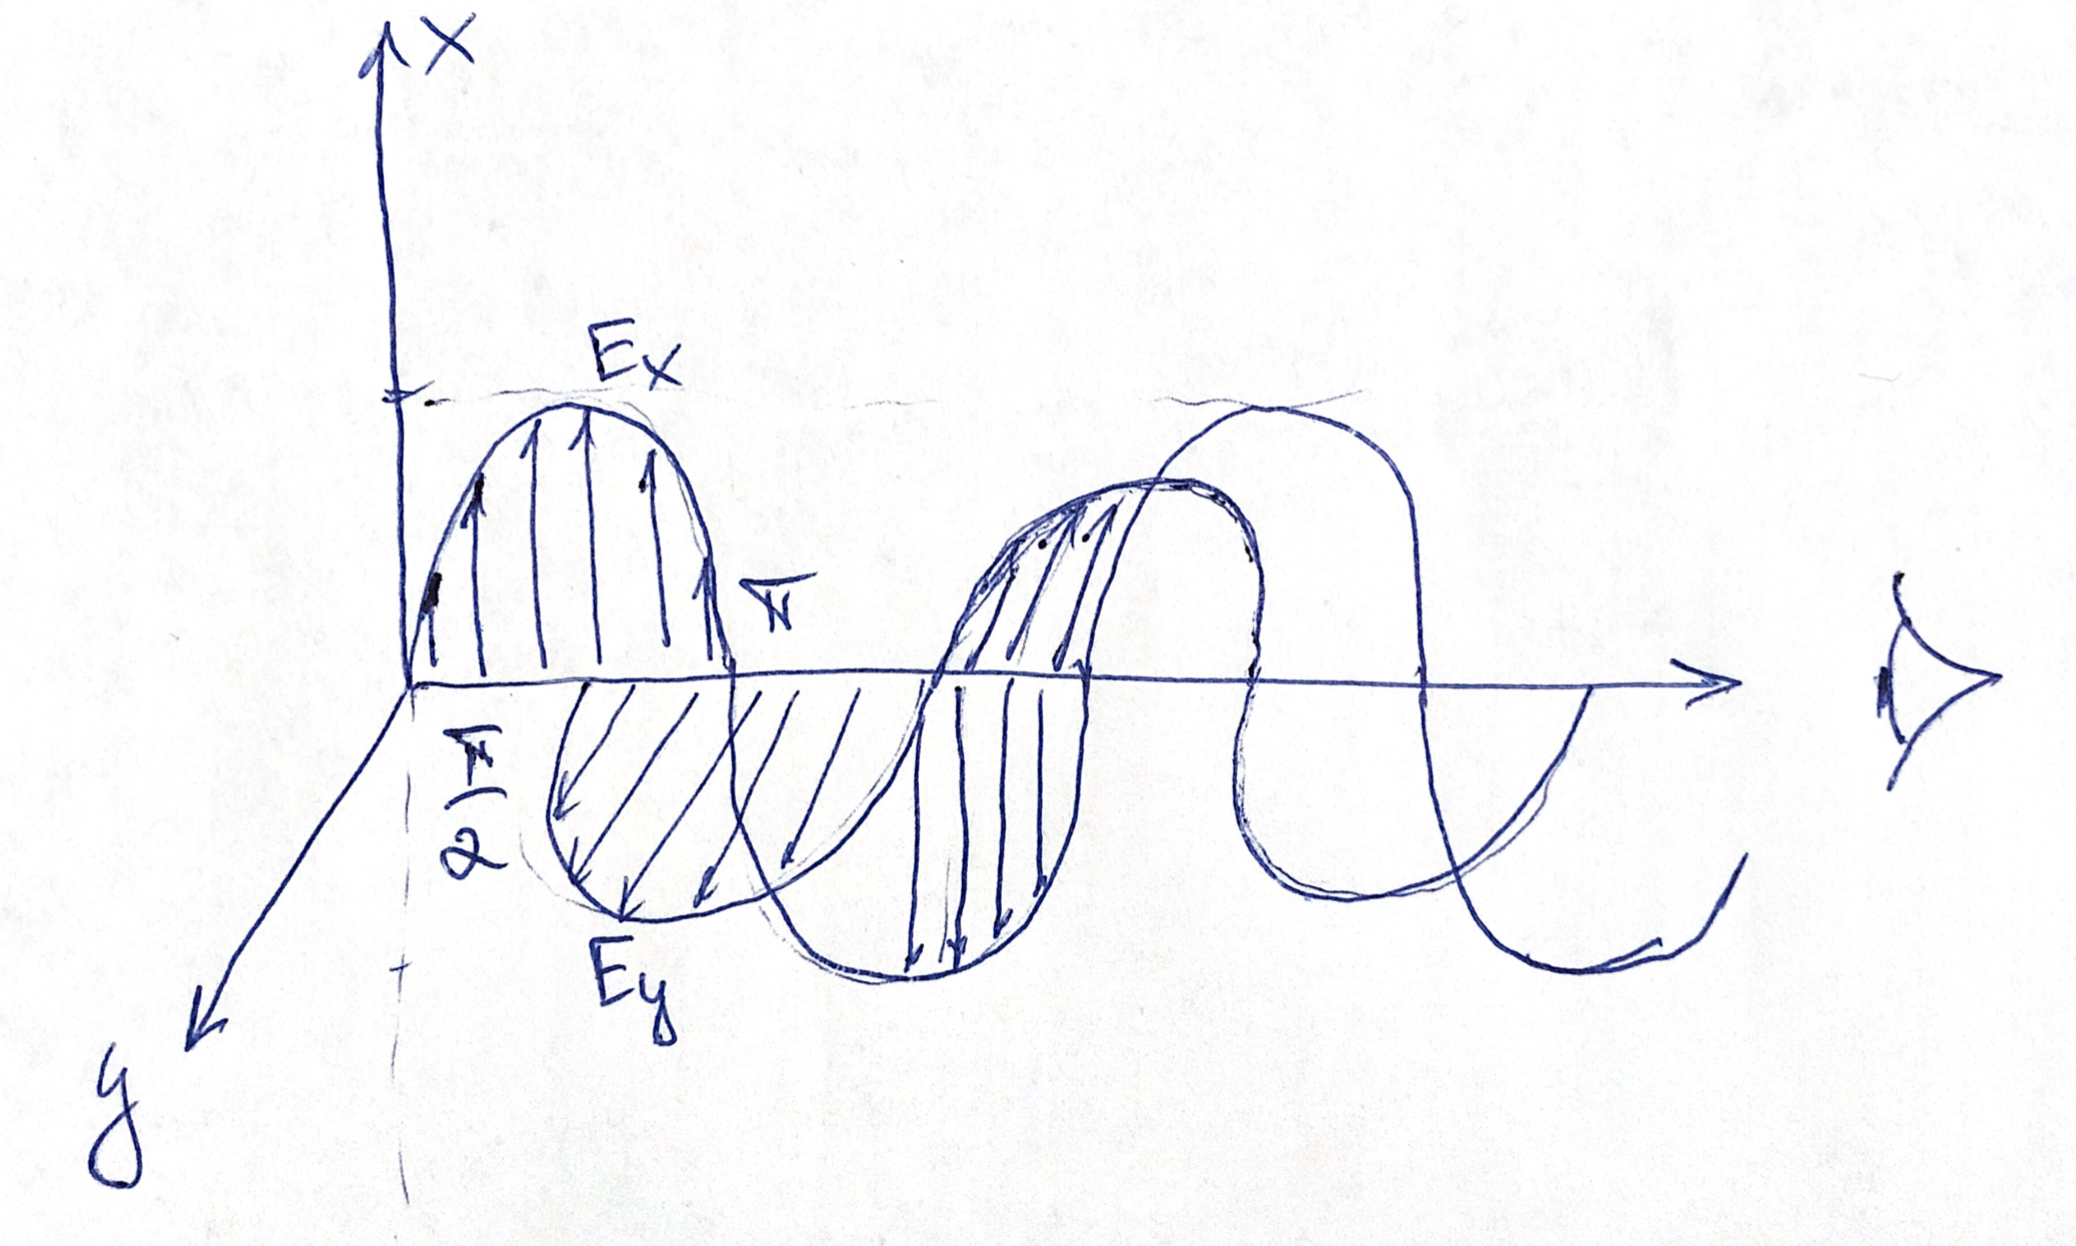
\includegraphics[width=1\linewidth]{waves.png}
\caption{Вышедшие из пластинки синусоиды} %% подпись к рисунку
\label{waves} %% метка рисунка для ссылки на него
\end{minipage}
\hfill 
\begin{minipage}[h]{0.4\linewidth}
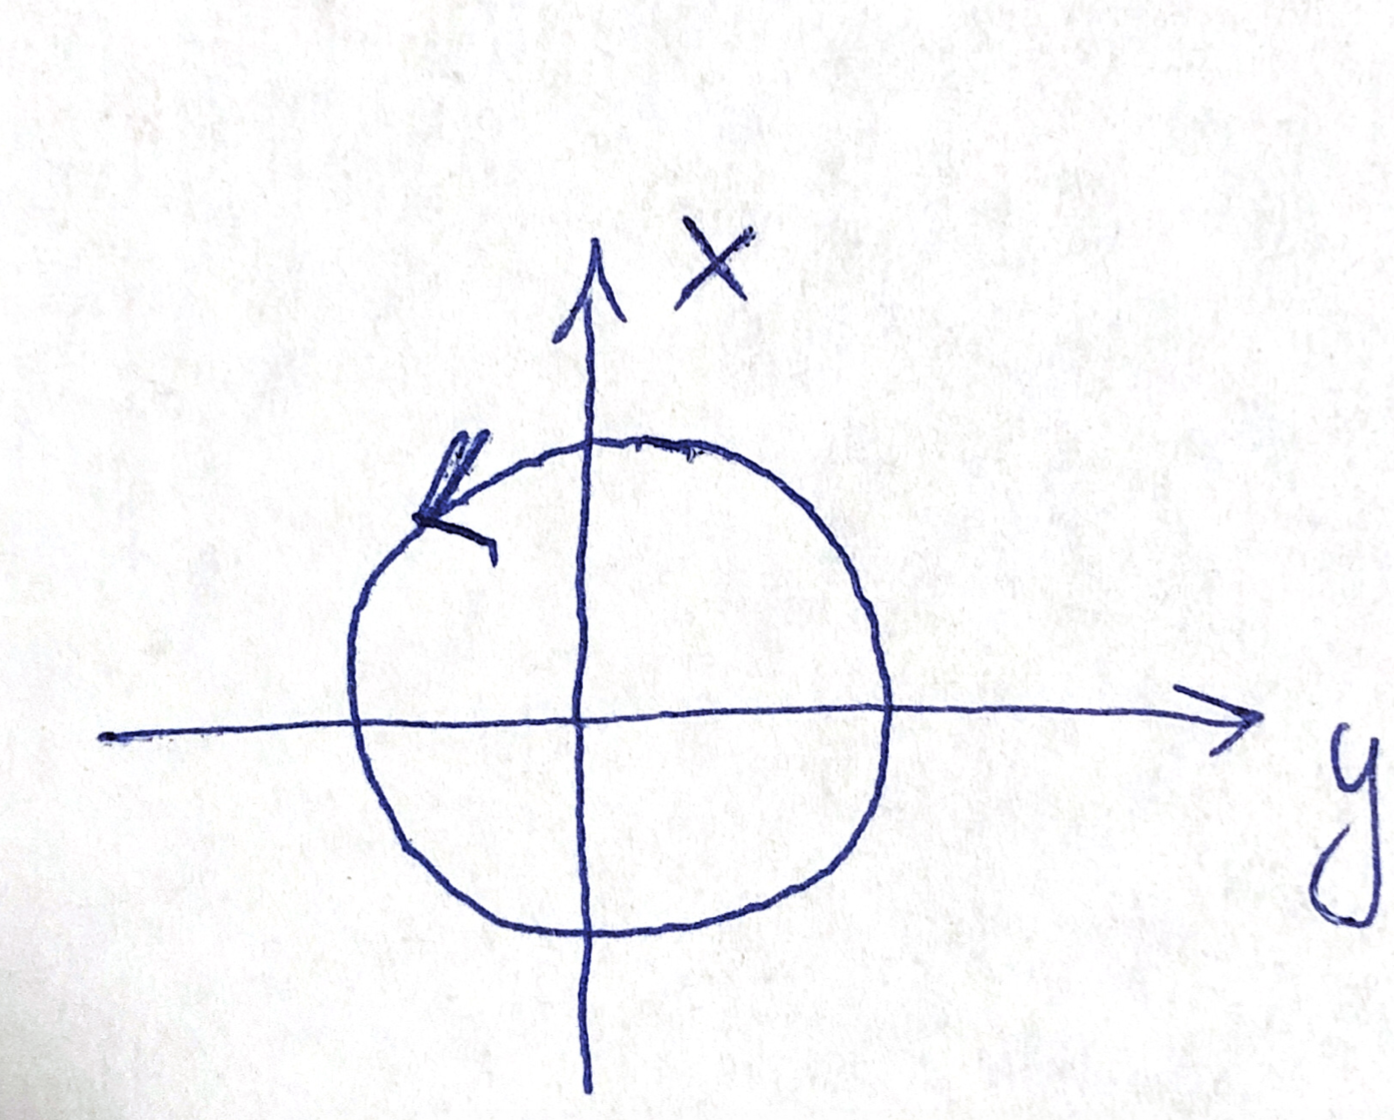
\includegraphics[width=1\linewidth]{direct.png}
\caption{Эллипс поляризации; ось $x$ соответсвует большей скорости}
\label{direct}
\end{minipage}
\end{center}
\end{figure}

\item  Для определения направления вращения светового вектора в эллипсе
установим между поляроидами дополнительную пластинку $\lambda/4$ с известными направлениями «быстрой» и «медленной» осей, ориентированными по осям эллипса поляризации анализируемого света.
В этом случае вектор $\vec{E}$ на выходе будет таким, как если бы свет прошёл две
пластинки $\lambda/4$: свет на выходе из второй пластинки будет линейно поляризован. Если пластинки поодиночке дают эллипсы, вращающиеся в разные стороны, то поставленные друг за другом, они скомпенсируют
разность фаз, и вектор $\vec{E}$ на выходе останется в первом
и третьем квадрантах. Если
же световой вектор перешёл в смежные квадранты, значит, эллипсы вращаются в одну сторону. 
\par После второго поляроида интенсивность света максимальна. Значит, две пластины усиливают друг друга, световой вектор перешёл в смежные квадранты, эллипсы вращаются в одну сторону.

\end{enumerate}


\section{Вывод}
Изучили свойства поляризованного света и на практике проверили оптические характеристики некоторых предметов и материалов.

\newpage

\section{Контрольные вопросы}


\textbf{Покажите, что при выполнении условий Брюстера отраженный и преломленный лучи взаимно перпендикулярны?}

\begin{wrapfigure}[12]{r}{130pt}
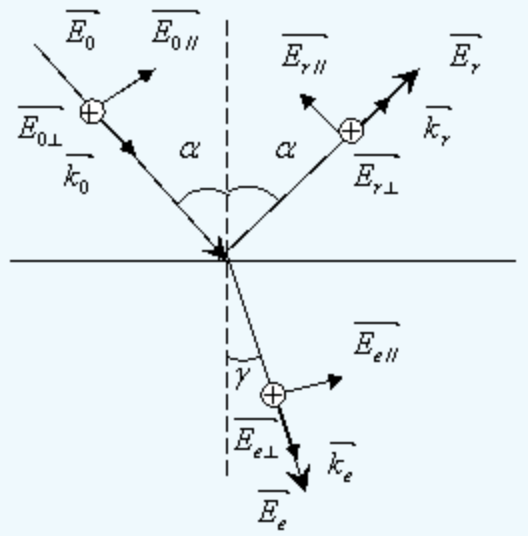
\includegraphics[scale = 0.4]{brust.png}
\caption{Закон Брюстера}
\label{brust}
\end{wrapfigure}

Степень поляризации отраженного и преломленного луча при различных углах падения получается из решения уравнении Максвелла с учетом условий на границе диэлектриков. (рис.\ref{brust})
К числу этих условий принадлежат: равенство тангенциальных составляющих векторов $\vec{E}$ и $\vec{H}$ по обе стороны границы раздела (с одной стороны нужно брать сумму соответствующих векторов для падающей и отраженной волны, с другой - вектор для преломленной волны) и равенство нормальных составляющих векторов $\vec{D}$ и $\vec{B}$

В результате получим следующие формулы:

\begin{center}
\begin{equation*}
\begin{cases}
   E_{r \|} = E_{o \|} \frac{\tg(\alpha - \gamma)}{\tg(\alpha + \gamma)} 
   \\
   E_{r \perp} = - E_{o\perp} \frac{\sin{(\alpha - \gamma)}}{\sin{(\alpha + \gamma)}}
\end{cases}
\end{equation*}
\end{center}

Из этих двух уравнений вытекает, что если $\alpha + \gamma = \pi/2$, то тогда $\tg(\alpha + \gamma) = \infty$ и $E_{r \|} = 0$. Значит, что в отраженном свете присутствуют только колебания $E_{r \perp}$. 


\


\textbf{Как отличить свет с правой и с левой круговой поляризацией?}

Это зависит от сдвига фаз между $E_x$ и  $E_y$. 

Если $E_y$ отстает на $\pi/2$ от $E_x$, то $\vec{E}$ вращается против часовой стрелки и значит, что это левая круговая поляризация как на рис.\ref{waves} 

Если $E_y$ опережает на $\pi/2$  $E_x$, то $\vec{E}$ вращается по часовой стрелки и значит, что это правая круговая поляризация. 

Можно вставлять $\lambda/4$ пластинку, чтобы получить линейную поляризацию с двумя разными наклонами в зависимости от первоначального направления поляризации. $\vec{E}$ лежит во 2 и 4 квадратурах, то это левая круговая. Если $\vec{E}$ лежит в 1 и 3 квадратурах, то это правая круговая. 


 

\textbf{Неполяризованный свет проходит через двоякопреломляющую пластинку $\lambda/4$. Что можно саказать о поляризации света на выходе из пластинки?}



Будут образованы 2 поляризованных луча. Двойное лучепреломление объясняется анизотропностью кристаллов. Диэлектрическая проницаемость зависит от направления. 


\begin{wrapfigure}[14]{r}{130pt}
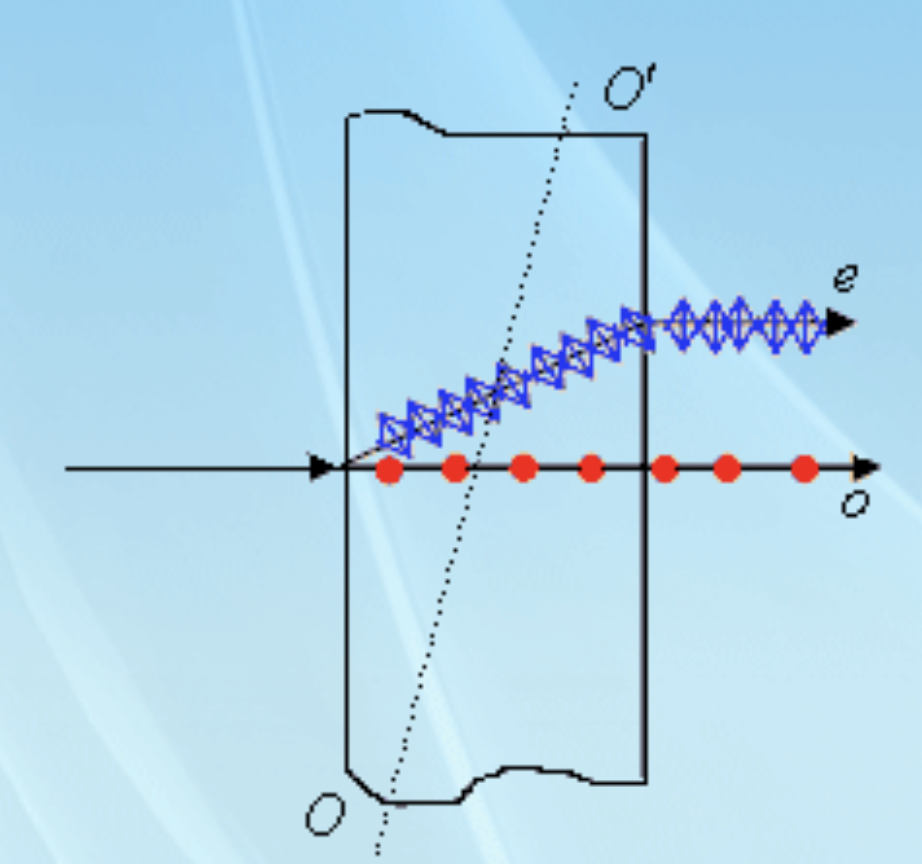
\includegraphics[scale = 0.25]{shpat.png}
\caption{e - необыкновенный; о - обыкновенный}
\label{shpat}
\end{wrapfigure}

Поэтому скорость световых волн будет зависеть от направления колебаний вектора $\vec{E}$. В обыкновенном луче колебаний вектора $E_x$ происходят в перпендикулярном направлении к главному сечению кристалла (плоскость проходящая через оптическую ось). Необыкновенный же луч будет иметь перпендикулярную компоненту $E_y \perp E_x$ (поскольку реч идет об одноосном кристалле). Ввиду разности коэффициентов преломлений вдоль двух направлений скорость распространения лучей будет разная, что приведет к набегу разности фаз. 



\

\

\

\

\textbf{Как отличить естественный свет от света, поляризованного по кругу, и от смеси естественного света со светом, поляризованного по кругу}

Как для поляризованного по кругу, так и для света естественного, интенсивность после прохождения через анализатор одинакова при любой его ориентации.

Чтобы отличить неполяризованный от поляризованного по кругу, нудно сдвинуть фазу между поляризациями преобразуя эллиптическую поляризацию в линейную, которуы в дальнейшем можно полностью погасить при определенной ориентации анализатора.  Это можно сделать с помощью системы двояколучепреломляющих пластинок, вырезанных параллельно главной оптической оси кристалла. У таких пластинок отличаются коэффициенты преломления для волн, поляризованных параллельно и перпендикулярно главной оси, что и приводит к изменению сдвига фаз между ними. 

Естественный свет можно рассматривать как наложение двух волн одинаковой интенсивности с ортогональными поляризациями, разность фаз между которыми изменяется в течение времени наблюдения случайно. Внесение четвертьволновой пластинкой дополнительной постоянной разности фаз между ними не может изменить случайного характера соотношения фаз ортогональных составляющих. Поэтому прошедший через четвертьволновую пластинку свет остается неполяризованным и его интенсивность не меняется при повороте анализатора. 

Степень поляризации можно определить для произвольно поляризованной волны:

$$P = \frac{I_{max}(\varphi , \delta) - I_{min}(\varphi , \delta)}{I_{max}(\varphi , \delta) + I_{min}(\varphi , \delta)}$$ 

где макс и мин значение интенсивности беруть уже не только при изменении угла поворота анализатор, но и при изменении разницы оптических длин путей в пластинке перед анализатором. 

\

\textbf{Объясните изменения интенсивности и цвета, наблюдаемые в опытах по интерференции поляризованных лучей}

Ответ в пункте 3.7. 


\

\textbf{Почему свет от вечернего неба поляризован?}

Это происходит из-за рассеяния света на препядствиях значительно меньших длины волны. Если солнце стоит в зените, то поляризация будет максимальна вдоль горизонта. А если солнце находится в горизонте, то максимальная поляризация достигается в направлении, перпендикулярном солнцу, проходящем через зенит. 

\begin{wrapfigure}[10]{r}{130pt}
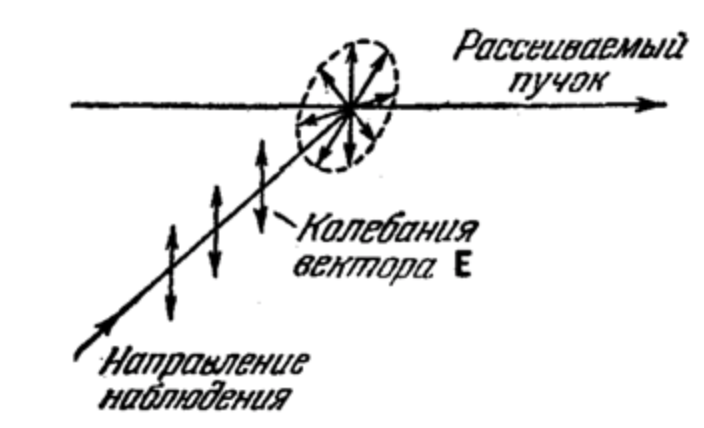
\includegraphics[scale = 0.4]{refl.png}
\caption{Поляризация}
\label{refl}
\end{wrapfigure}

Рассеиваемый пучок света вызывает в частицах колебания зарядов, направления которых лежат в плоскости, перпендикулярной к пучку (рис.\ref{refl}). Колебания вектора $\vec{E}$ во вторичной волне происходят в плоскости, проходящей через направление колебаний зарядов. Поэтому свет, рассеиваемый частицами в направлениях, перпендикулярных к пучку, будет полностью поляризован. В направлениях, образующих с пучком угол, отличный от $\pi/2$, рассеянный свет поляризован только частично. 







\end{document}